\documentclass[11pt]{article}

% ---------- Packages ----------
\usepackage[margin=1in]{geometry}
\usepackage{amsmath, amssymb}
\usepackage{graphicx}
\usepackage{fancyhdr}
\usepackage{float}
\usepackage{listings}
\usepackage{xcolor}
\usepackage{cancel}
\usepackage[normalem]{ulem}

% ---------- MATLAB Code Listing Style ----------
\lstdefinestyle{matlab}{
    language=Matlab,
    basicstyle=\ttfamily\footnotesize,
    breaklines=true,
    breakatwhitespace=false,
    postbreak=\mbox{$\hookrightarrow$\space},
    columns=fullflexible,
    keepspaces=true,
    frame=none,
    numbers=left,
    numberstyle=\tiny,
    showstringspaces=false
}
\lstset{style=matlab}

% ---------- Paragraph Formatting ----------
\setlength{\parindent}{0pt}
\setlength{\parskip}{0.5em}

% ---------- Header ----------
\pagestyle{fancy}
\fancyhf{}
\lhead{ASEN 5335 Aerospace Environment}
\rhead{Justin Le}
\cfoot{\thepage}

% ---------- Document ----------
\begin{document}

% ---------- Title ----------
\begin{center}
    {\Large \textbf{Homework 3}}\\[0.5em]
    {\large ASEN 5335 Aerospace Environment}\\[0.5em]
    Justin Le\\ 
    \today
    \\[0.5em]
\end{center}

\vspace{1em}
\section*{Problem 1: Plotting the Ionosphere}
\subsection*{(i.)}

\begin{figure}[H]
    \centering
    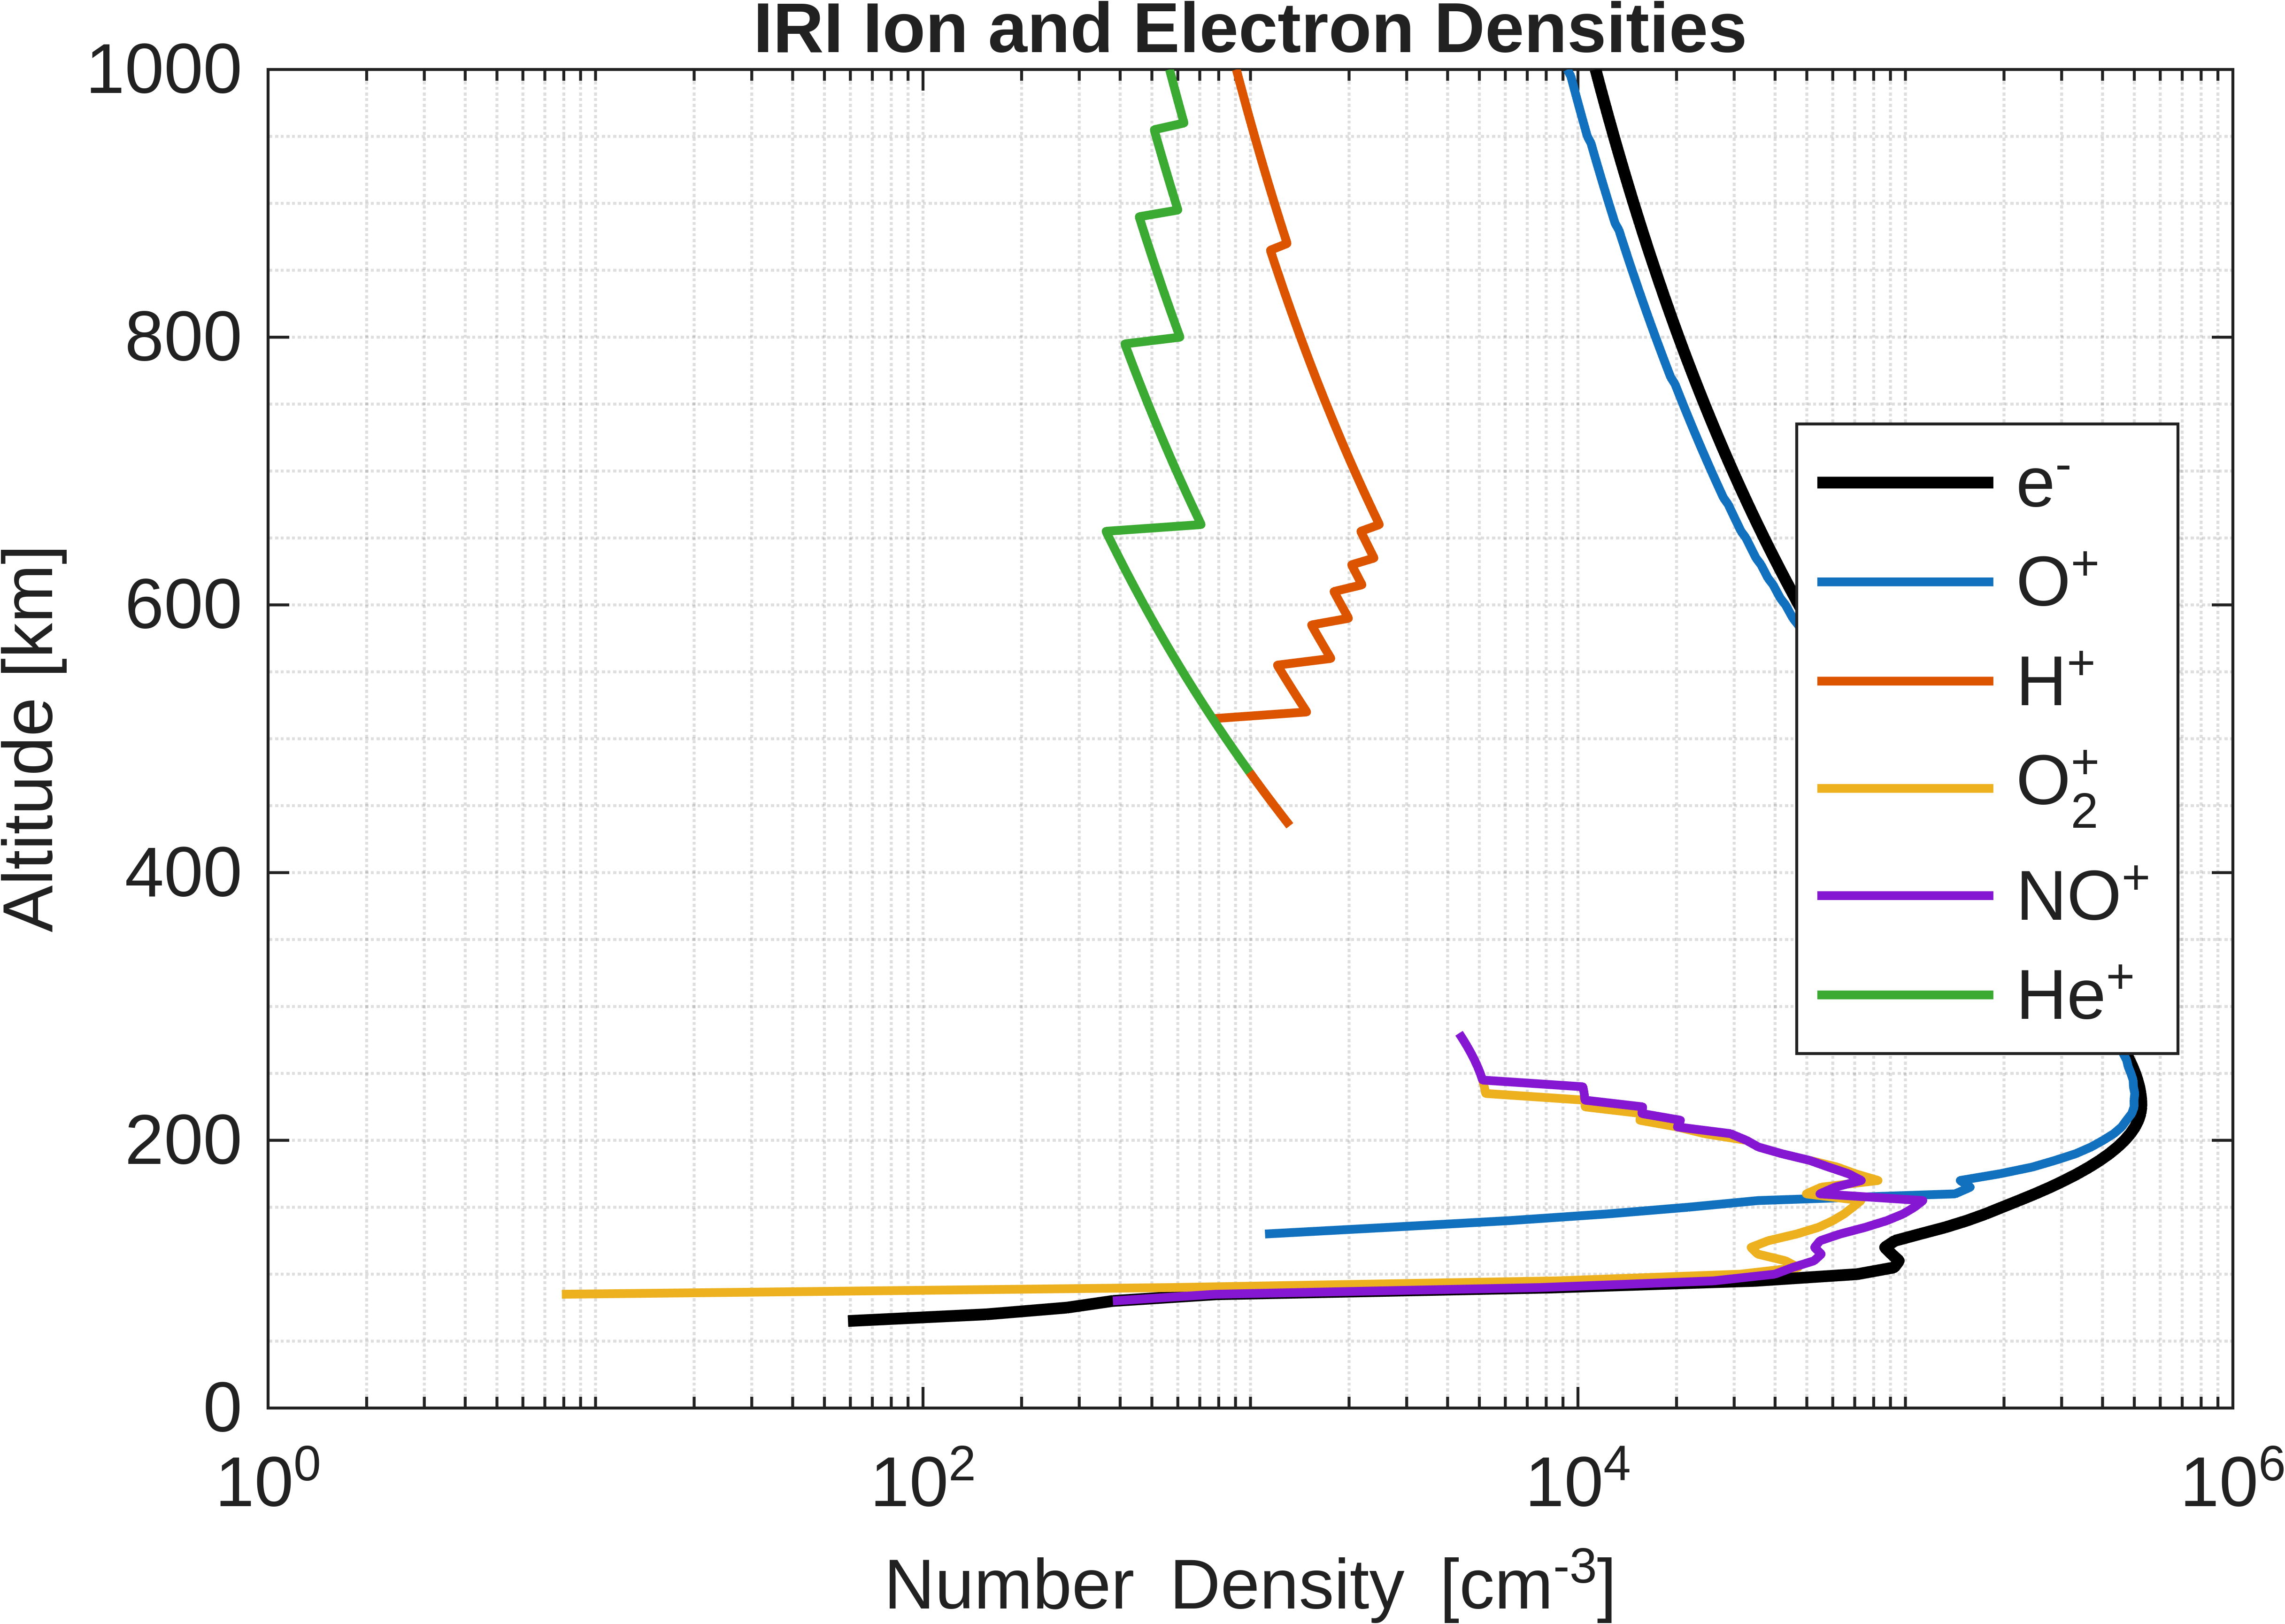
\includegraphics[width=0.6\textwidth]{figures/HW3_P1_iri_output.png}
    \caption{IRI Output}
    \label{fig:iri_output}
\end{figure}

\begin{figure}[H]
    \centering
    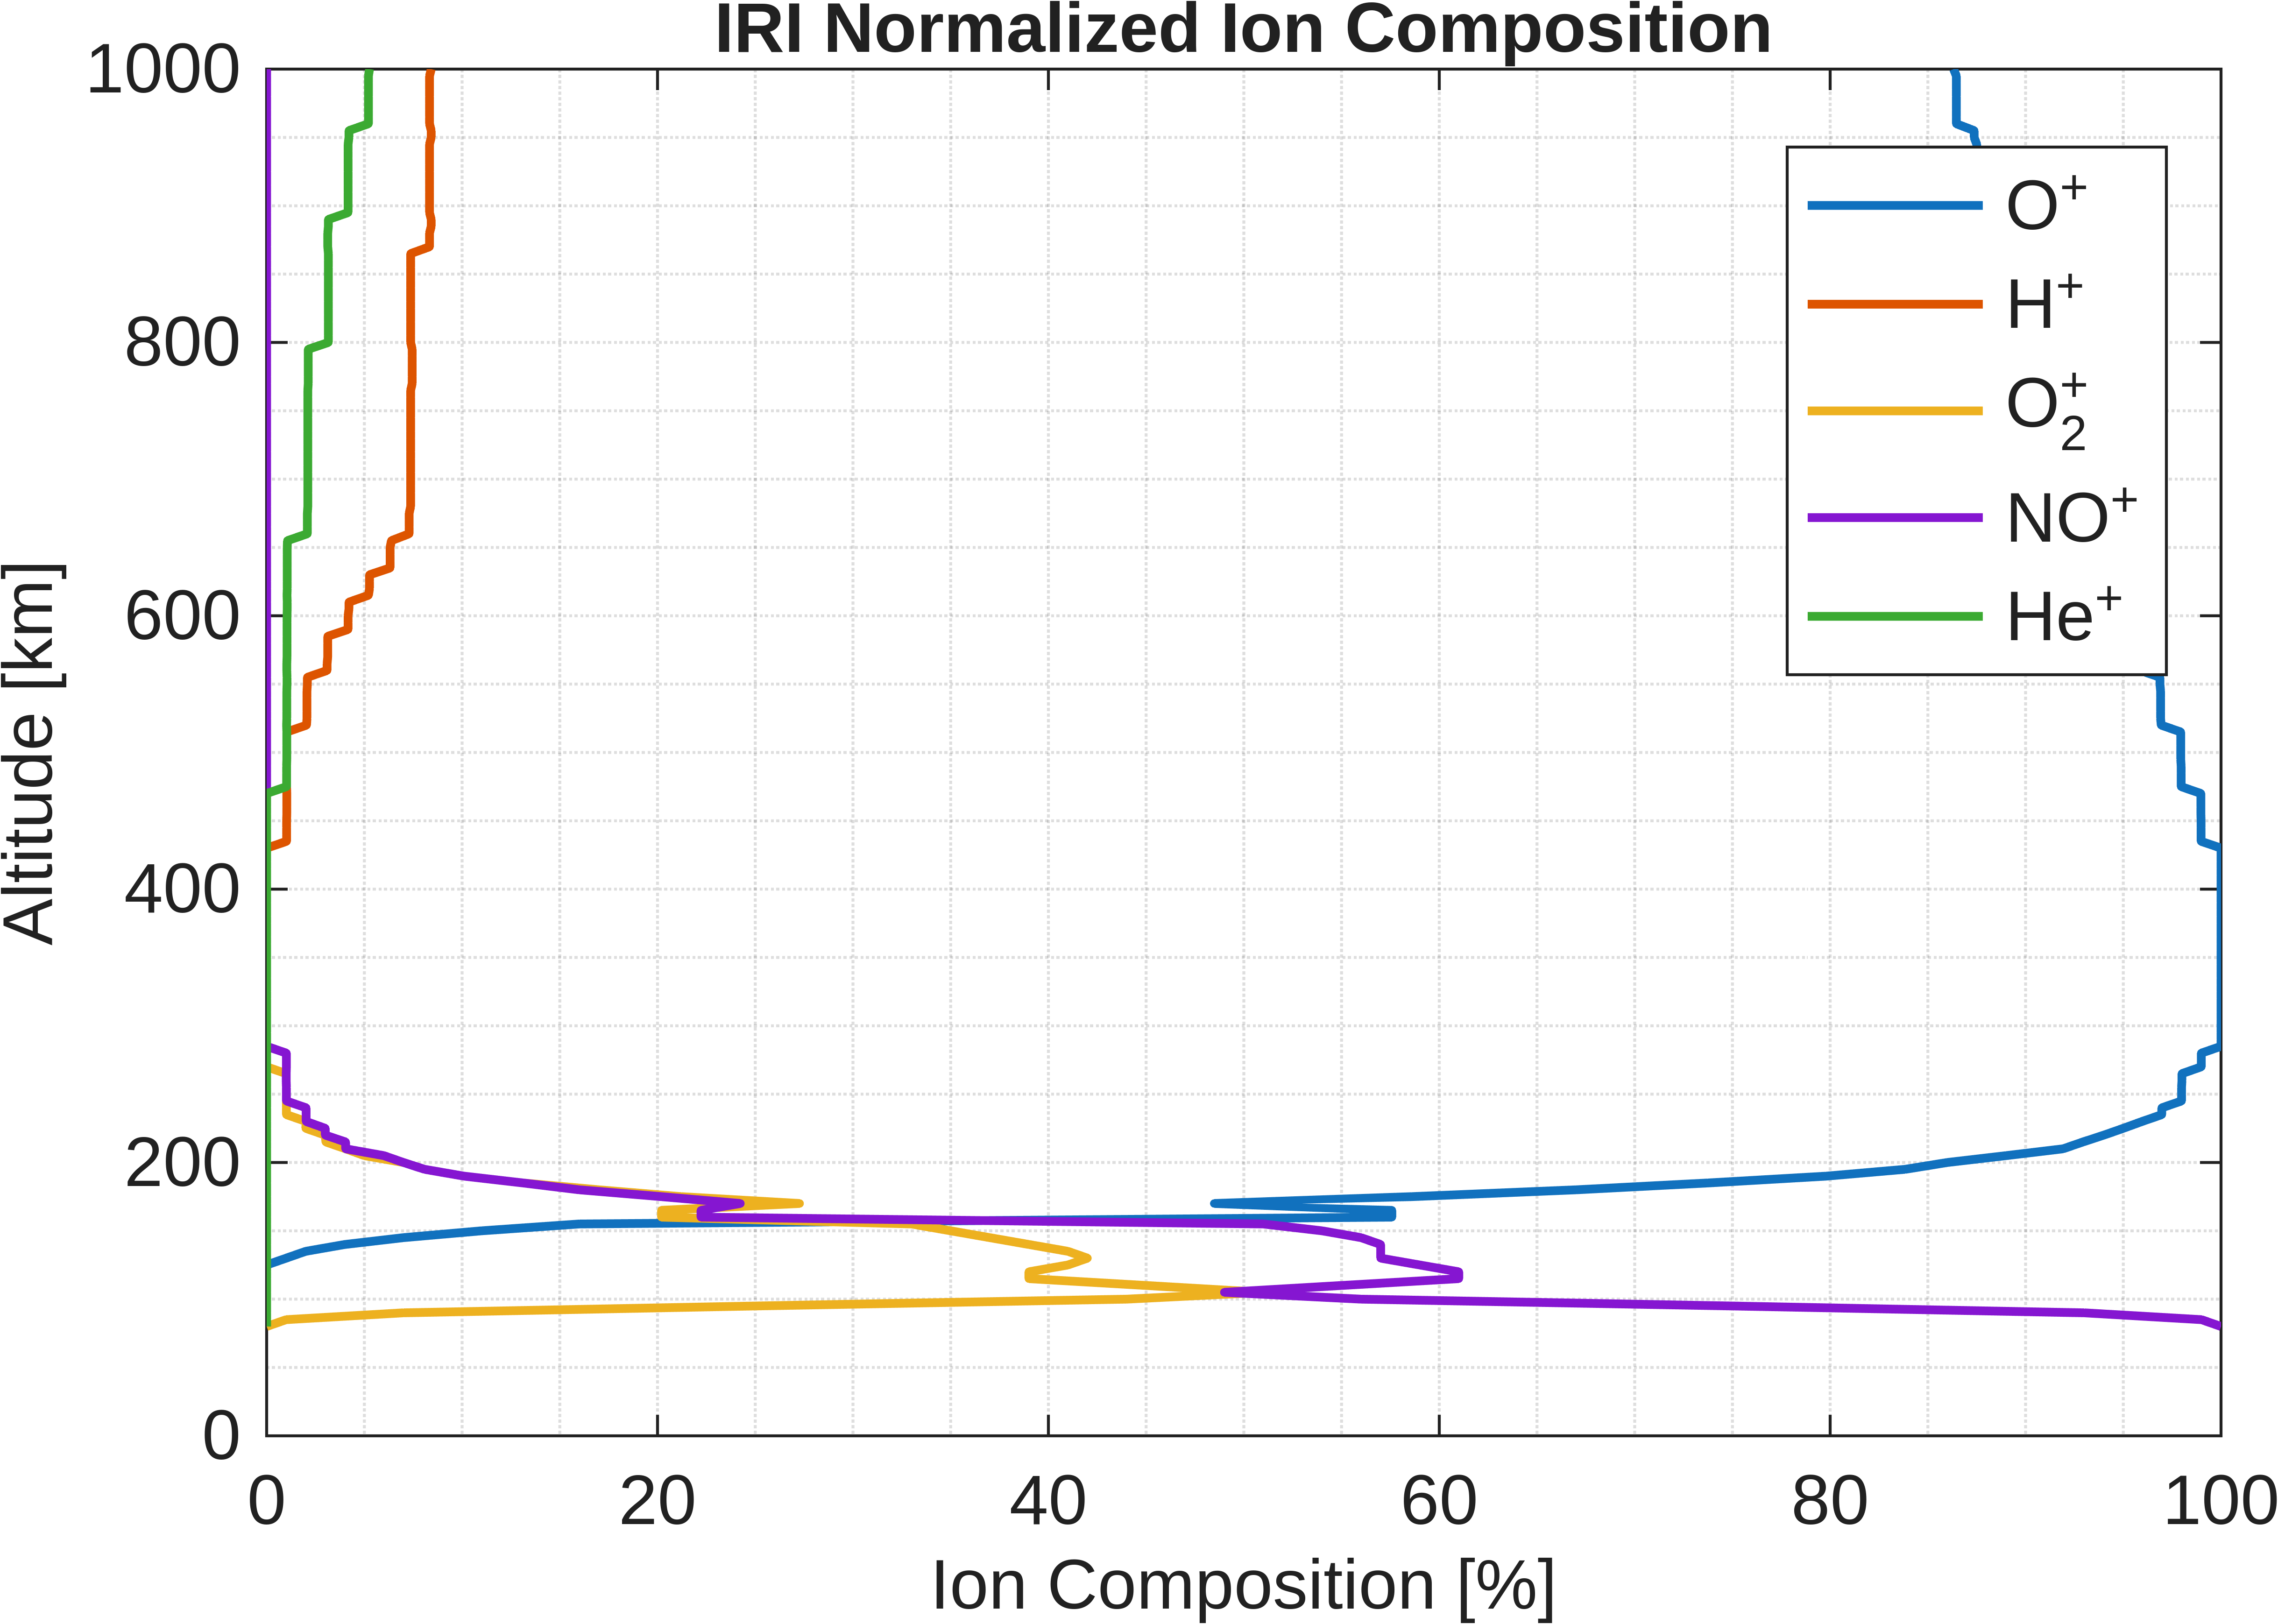
\includegraphics[width=0.6\textwidth]{figures/HW3_P1_ion_composition.png}
    \caption{IRI Output Normalized}
    \label{fig:iri_output_normalized}
\end{figure}

\subsection*{(ii.)}
\hspace*{2em}Below 500 km, we can observe that $NO^+$ dominates between \sout{0-160 km} \textcolor{red}{80-155 km}. $O_2^+$ contributes more than 20\% at
between \sout{90} \textcolor{red}{95} and 175 km.

\hspace*{2em}\textcolor{red}{The IRI output has no ion composition below 80 km, so the lower bound starts there. $O^+$ takes over
at 160 km. At 90 km $O_2^+$ is only 7\% and reaches 25\% at 95 km.}

\subsection*{(iii.)}
\hspace*{2em}By convention 1 TECU is $10^{16}\,\mathrm{el/m^2}$. Integrating the total electrons from the IRI
output, we find the TEC of the entire IRI output to be 12.47 TECU. \sout{When the peak electron density is $525696\,\mathrm{m^{-3}}$, we can integrate
the topside and bottomside seperately to find they are 3.55 TECU and 8.92 TECU respectively. Normalizing against the total TEC found, we find they are
28.49\% and 71.51\% respectively.}

\hspace*{2em}\textcolor{red}{The peak electron density is $525696\,\mathrm{cm^{-3}}$ ($5.26\times10^{11}\,\mathrm{m^{-3}}$) at 225 km. Using the peak as the boundary,
we integrate the topside and bottomside to find they are 8.92 TECU and 3.55 TECU respectively.
Normalizing against the total TEC found, the topside is 71.51\% and the bottomside is 28.49\%. This agrees with the IRI output, which gives 72\% of the
TEC above the F peak.}

\newpage
\section*{Problem 2: Peak Ionization}
\subsection*{(i.)}
\subsubsection*{E Region}
We are able to use the Chapman relation equation,
\begin{gather*}
n_e(z,\theta) = \left(\frac{q_{max}}{\alpha_{eff}}\right)^{1/2} \exp\!\left[\frac{1}{2}\left(1 - z_1 - e^{-z_1}\right)\right] \\
\text{Solving for $q_{max}$,} \\
q_{max} = \alpha_{eff}\, n_e^2 \exp\!\left[-\left(1 - z_1 - e^{-z_1}\right)\right] \\
\text{At the peak altitude $z = z_{max}$, $z_1 = 0$, so the exponential term is 1 and $n_e = n_{e,max}$:} \\
q_{max} = \alpha_{eff}\, n_{e,max}^2 \\
q_{max_E} = (10^{-8})(1.5\times10^{5})^2 \\
\boxed{q_{max_E}= 225~\mathrm{cm^{-3}\,s^{-1}}}
\end{gather*}
\subsubsection*{F1 Region}
Repeat the calculation above for the F1 Region,
\begin{gather*}
q_{max_F1} = (7\times10^{-9})(2.5\times10^{5})^2 \\
\boxed{q_{max_F1}= 437.5~\mathrm{cm^{-3}\,s^{-1}}}
\end{gather*}
\subsubsection*{F2 Region}
Repeat the calculation above for the F2 Region,
\begin{gather*}
q_{max_F2} = (5\times10^{-9})(5.0\times10^{5})^2 \\
\boxed{q_{max_F2}= 1250~\mathrm{cm^{-3}\,s^{-1}}}
\end{gather*}

\subsection*{(ii.)}
The reason why the ionization peak altitude $z_{max}$ moves upwards with increasing solar zenith angle
$\chi$ when all other factors are kept constant is because when examining the equation, \textcolor{red}{we notice that as $\chi$ increases,
the solar radiation propogates through a longer sland path through the atmosphere vs $\chi=0$. The energy is deposited and ionizes based on 
the total amount of atmosphere traversed. Energy is deposited in higher altitudes as the amount of atmosphere it travels through increases
with $\chi$. }


\newpage
\section*{Problem 3: Spacecraft Charging in LEO}
\hspace*{2em}We are able to use the charging equation,

\begin{gather*}
\frac{dQ}{dt} = I_e + I_i + I_{SEE,i} + I_b + I_{ph}
\end{gather*}

\hspace*{2em}By assuming $\frac{dQ}{dt} = 0$, the eclipse term, $I_{ph}=0$, 
and no secondary electron emission or backscattered electron current, $I_{SEE,i} = I_b = 0$, the equation simplifies to,

\begin{gather*}
0 = I_e + I_i
\end{gather*}

\hspace*{2em}Using equations for $I_i$, and $I_e$,
\begin{gather*}
I_i = q n_i v_{0} A_i \\
I_e = -\frac{1}{4} q n_e v_{e,th} A_e e^{qV/kT_e}
\end{gather*}

\hspace*{2em}and calculating 
\begin{gather*}
V_{fl} = \frac{k_B T_e}{q}\ln\left(\frac{4 v_0 A_i}{v_{e,th} A_e}\right)
\end{gather*}

\hspace*{2em}The thermal voltage at a constant $T_e = 1000\,\mathrm{K}$ is,
\begin{gather*}
\frac{k_B T_e}{q} = \frac{(1.381\times10^{-23}\,\mathrm{J/K})(1000\,\mathrm{K})}{1.602\times10^{-19}\,\mathrm{C}} = 0.0862\,\mathrm{V}
\end{gather*}

\hspace*{2em}The orbital velocity at $400\,\mathrm{km}$ altitude is,
\begin{gather*}
v_0 = \sqrt{\frac{\mu}{R_E + h}} = \sqrt{\frac{3.986\times10^{14}\,\mathrm{m^3/s^2}}{6.378\times10^{6}\,\mathrm{m} + 4.0\times10^{5}\,\mathrm{m}}} = 7.67\,\mathrm{km/s}
\end{gather*}

\hspace*{2em}The electron thermal velocity is,
\begin{gather*}
v_{e,th} = \sqrt{\frac{3 k_B T_e}{m_e}} = \sqrt{\frac{3(1.381\times10^{-23}\,\mathrm{J/K})(1000\,\mathrm{K})}{9.109\times10^{-31}\,\mathrm{kg}}} = 213\,\mathrm{km/s}
\end{gather*}

\hspace*{2em}If this is a 6U Cubesat, ions are collected
only on the $20 \times 30\,\mathrm{cm}$ ram face, electrons collect over entire surface,
\begin{gather*}
A_i = (0.2\,\mathrm{m})(0.3\,\mathrm{m}) = 0.06\,\mathrm{m^2} \\
A_e = 2(0.02\,\mathrm{m^2} + 0.03\,\mathrm{m^2} + 0.06\,\mathrm{m^2}) = 0.22\,\mathrm{m^2}
\end{gather*}

\hspace*{2em}Plug into the floating potential equation,
\begin{gather*}
\frac{4 v_0 A_i}{v_{e,th} A_e} = \frac{4(7.67\,\mathrm{km/s})(0.06\,\mathrm{m^2})}{(213\,\mathrm{km/s})(0.22\,\mathrm{m^2})} = 0.0392 \\
V_{fl} = (0.0862\,\mathrm{V})\ln(0.0392) = (0.0862\,\mathrm{V})(-3.24) \\
\boxed{V_{fl} \approx -0.28\,\mathrm{V}}
\end{gather*}

\hspace*{2em}My assumptions were equilibrium ($\frac{dQ}{dt} = 0$), eclipse ($I_{ph} = 0$), no secondary or backscattered
electrons, $n_e = n_i$, ions collected only on the ram face, electrons collected on the entire surface, and a
$10 \times 20 \times 30$ cm CubeSat in a circular orbit. We assume that the spacecraft is spherical in order to use the equations however
it should be noted that we still use the area of the 6U CubeSat provided. 

\newpage
\section*{Problem 4: Spacecraft Charging in GEO}
\hspace*{2em}Use the charging equation,
\begin{gather*}
\frac{dQ}{dt} = I_e + I_i + I_{SEE,i} + I_b + I_{ph}
\end{gather*}

\hspace*{2em}Assume $\frac{dQ}{dt} = 0$ and $I_{SEE,i} = I_b = 0$,
\begin{gather*}
0 = I_e + I_i + I_{ph}
\end{gather*}

\hspace*{2em}The electron current is,
\begin{gather*}
I_e = -\frac{1}{4} q n_e v_{e,th} A_e e^{qV/k_B T_e} \quad \text{for } V < 0 \\
I_e = -\frac{1}{4} q n_e v_{e,th} A_e \left(1 + \frac{qV}{k_B T_e}\right) \quad \text{for } V > 0
\end{gather*}

\hspace*{2em}The ion current is,
\begin{gather*}
I_i = \frac{1}{4} q n_i v_{i,th} A_i e^{-qV/k_B T_i} \quad \text{for } V > 0 \\
I_i = \frac{1}{4} q n_i v_{i,th} A_i \left(1 - \frac{qV}{k_B T_i}\right) \quad \text{for } V < 0
\end{gather*}

\hspace*{2em}The photocurrent from a sunlit surface is,
\begin{gather*}
I_{ph} = \left(40~\mathrm{\frac{\mu A}{m^2}}\right) A\cos\theta\, e^{-qV/k_B T_{ph}}, \qquad k_B T_{ph} \simeq 2~\mathrm{eV}
\end{gather*}

\hspace*{2em}$n_e = n_i = 0.5~\mathrm{cm^{-3}}$, $T_e = T_i = 5\times10^{6}~\mathrm{K}$, and $A_i = A_e = A$ so the area cancels.
The thermal voltage and thermal velocities are,
\begin{gather*}
\frac{k_B T}{q} = \frac{(1.381\times10^{-23}\,\mathrm{J/K})(5\times10^{6}\,\mathrm{K})}{1.602\times10^{-19}\,\mathrm{C}} = 431\,\mathrm{V} \\
v_{e,th} = \sqrt{\frac{3 k_B T_e}{m_e}} = 1.51\times10^{4}\,\mathrm{km/s} \\
v_{i,th} = \sqrt{\frac{3 k_B T_i}{m_i}} = 352\,\mathrm{km/s}
\end{gather*}

\subsection*{Shadow Surface}
\hspace*{2em}In shadow $I_{ph} = 0$ and $V < 0$, the electron and ion currents for $V<0$,
\begin{gather*}
0 = -\frac{1}{4} q n_e v_{e,th} e^{qV/k_B T_e} + \frac{1}{4} q n_i v_{i,th}\left(1 - \frac{qV}{k_B T_i}\right)
\end{gather*}
\hspace*{2em}Solving numerically with MATLAB,
\begin{gather*}
\boxed{V_{shadow} \approx -1079\,\mathrm{V}}
\end{gather*}

\subsection*{Sunlit Surface}
\hspace*{2em}In sunlight $V > 0$, and assuming $\cos\theta = 1$ and $k_B T_{ph} \simeq 2~\mathrm{eV}$,
\begin{gather*}
0 = -\frac{1}{4} q n_e v_{e,th}\left(1 + \frac{qV}{k_B T_e}\right) + \frac{1}{4} q n_i v_{i,th} e^{-qV/k_B T_i} + \left(40~\mathrm{\frac{\mu A}{m^2}}\right) e^{-qV/k_B T_{ph}}
\end{gather*}
\hspace*{2em}Solving numerically with MATLAB,
\begin{gather*}
\boxed{V_{sun} \approx 9.8\,\mathrm{V}}
\end{gather*}

\subsection*{Potential Difference}
\begin{gather*}
\Delta V = V_{sun} - V_{shadow} = 9.8\,\mathrm{V} - (-1079\,\mathrm{V}) \\
\boxed{\Delta V \approx 1089\,\mathrm{V}}
\end{gather*}

\newpage
\section*{Problem 5: Radio Wave Propagation}
\subsection*{(i.)}
\hspace*{2em}To find the minimum radio frequency to communicate from ground
to space, we would need the frequency that exceeds the largest critical frequency in 
the atmosphere. The critical frequency (with $n_e$ in cm$^{-3}$) is,
\begin{gather*}
f_c = 9\times10^{-3}\sqrt{n_e}~\mathrm{MHz} \\
\textcolor{red}{\text{Using the peak electron density from the IRI output, } n_{e,max} = 525696~\mathrm{cm^{-3}}} \\
\textcolor{red}{f_c = 9\times10^{-3}\sqrt{525696}} \\
\boxed{f_c = 6.53~\mathrm{MHz}}
\end{gather*}
\hspace*{2em}\textcolor{red}{Frequencies above 6.53 MHz will be able to transmit through the ionosphere into space.}
\subsection*{(ii.)}
\hspace*{2em}To find the region where this frequency Reflectsr, \sout{we need to find the region where
radio waves are below this frequency.} \textcolor{red}{we find the altitude of the peak electron density. The critical frequency would be at}
$\boxed{\cancel{\text{below }225~\mathrm{km}}}$ $\boxed{\textcolor{red}{225~\mathrm{km}}}$\textcolor{red}{, which would be the F2 region.}

\subsection*{(iii.)}
\hspace*{2em}To find the region where $2~\mathrm{MHz}$ signal would reflect, we would treat that
frequency as the critical frequency to find in the IRI output. \textcolor{red}{This gives
$n_e = \left(\frac{2}{9\times10^{-3}}\right)^2 = 49383~\mathrm{cm^{-3}}$, which occurs at two altitudes.
For ground-to-space transmission,} this would occur at about $\boxed{97~\mathrm{km}}$,
which would be the \sout{D region} \textcolor{red}{lower E region}. \textcolor{red}{For space-to-ground transmission, the wave
reflects on the topside at about} $\boxed{\textcolor{red}{592~\mathrm{km}}}$\textcolor{red}{.}

\begin{figure}[H]
    \centering
    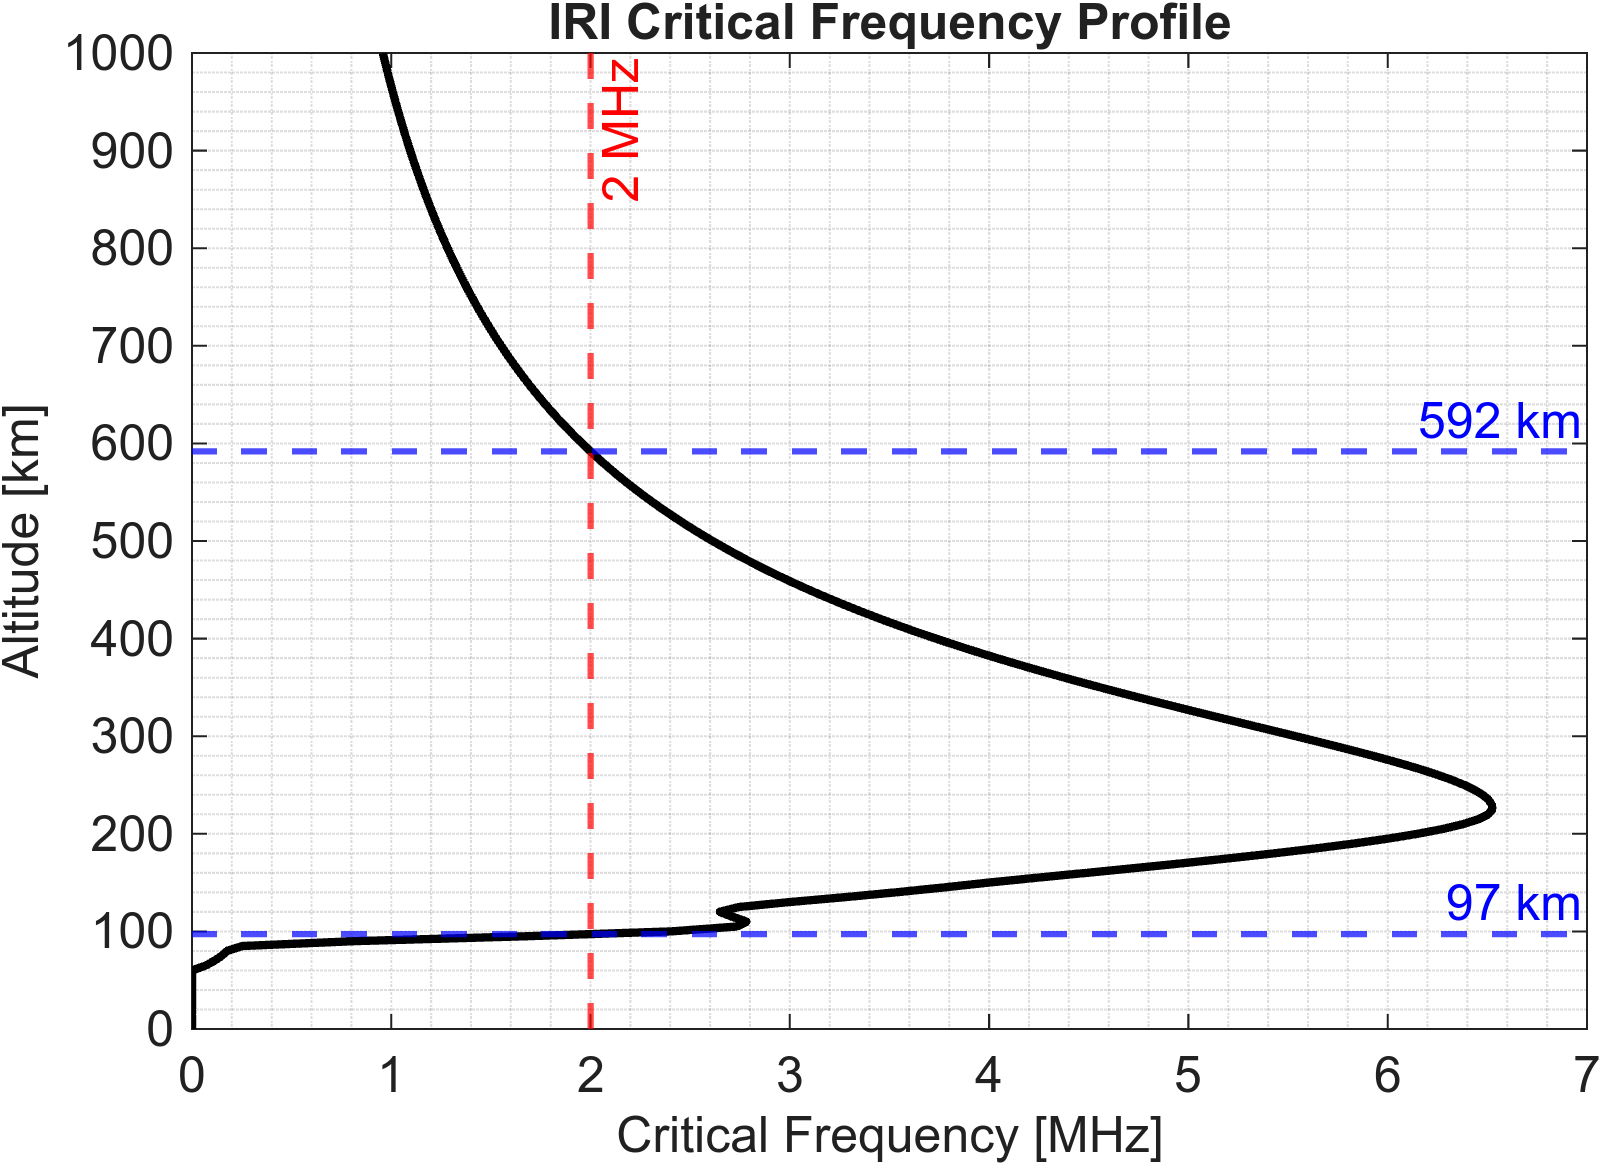
\includegraphics[width=0.6\textwidth]{figures/HW3_P5_plasma_freq_rev.png}
    \caption{IRI Critical Frequency}
    \label{fig:IRI Plasma Frequency}
\end{figure}

\newpage
\section*{Problem 6: Radio Blackout}
\subsection*{(i).}
\hspace*{2em}The reason that the spacecraft temporarily loses the ability to communicate
with the ground is because during re-entry, there is an envelope of ionized atmosphere around
the spacecraft, due to the re-entry processes' heat generated. This envelope of ionized atmosphere would
have some plasm frequency that would cause radio signals to reflect, causing this radio blackout.
\subsection*{(ii).}
\hspace*{2em}If the module module communicates with the ground at $2282.5~\mathrm{MHz}$, to find
the electron density in the plasma sheath region, we use the equation,
\begin{gather*}
f_c = 9\times10^{-3}\sqrt{n_{ec}} \\
\text{rewrite for } n_{ec} \text{,}\\
n_{ec} = (\frac{f_c}{9\times10^{-3}})^2 \\
n_{ec} = \left(\frac{2282.5}{9\times10^{-3}}\right)^2 = 6.432\times10^{10}~\mathrm{cm^{-3}} \\
\boxed{n_{ec} = 6.432\times10^{16}~\mathrm{m^{-3}}}
\end{gather*}

\newpage
\section*{Problem 7: GPS Delays}
\subsection*{(i).}
\hspace*{2em}We seek the path length delay through the ionosphere for 10 TECU using,
$L1 = 1575.42~\mathrm{MHz}$ and $L2 = 1227.60~\mathrm{MHz}$, we can use the equation,
\begin{gather*}
\Delta l_{iono} = -\frac{40.3}{f^2}TEC \\
\text{where } TEC = 10~\mathrm{TECU} = (10)(10^{16}~\mathrm{el/m^2}) = 10^{17}~\mathrm{el/m^2} \\
\Delta l_{iono L1} = -\frac{(40.3)(10^{17}~\mathrm{el/m^2})}{(1575.42\times10^{6}~\mathrm{Hz})^2} \\
\boxed{\Delta l_{iono L1} = -1.62~\mathrm{m}}\\
\Delta l_{iono L2} = -\frac{(40.3)(10^{17}~\mathrm{el/m^2})}{(1227.60\times10^{6}~\mathrm{Hz})^2} \\
\boxed{\Delta l_{iono L2} = -2.67~\mathrm{m}}
\end{gather*}
\subsection*{(ii).}
\hspace*{2em}We are able to use multiple frequencies because of the fact that ionospheric
delay depends on frequencies. By modeling two frequencies provided by GPS satellites, we can
then account for these ionospheric errors. By reducing this increased path due to the 
ionosphere, we can improve our pseudoranging and have a better position estimate.

\begin{gather*}
\textcolor{red}{L_i = s_i - \frac{40.3}{f_i^2}TEC} \\
\textcolor{red}{L_1 - L_2 = \left[s_1 - \frac{40.3}{f_1^2}TEC\right] - \left[s_2 - \frac{40.3}{f_2^2}TEC\right]} \\
\textcolor{red}{L_1 - L_2 = 40.3\,TEC\left(\frac{1}{f_2^2} - \frac{1}{f_1^2}\right) = 40.3\,TEC\,\frac{f_1^2 - f_2^2}{f_1^2 f_2^2}} \\
\textcolor{red}{\text{Solving for TEC,}} \\
\textcolor{red}{\boxed{TEC = \frac{f_1^2 f_2^2 \left(L_1 - L_2\right)}{40.3\left(f_1^2 - f_2^2\right)}}}
\end{gather*}
\hspace*{2em}\textcolor{red}{With TEC the ionospheric delay
$\frac{40.3}{f_i^2}TEC$ on each frequency can be computed and removed.}

\newpage
\section*{Problem 8: D Region Signal Attenuation}
\hspace*{2em}The electron-neutral collision frequency is found from the MSIS neutral density \sout{and the IRI electron temperature,}
\textcolor{red}{relative to the neutral density at the surface of the Earth,}
\begin{gather*}
\cancel{\nu_{en} = 5.4\times10^{-10}\, n_n T_e^{1/2}~\mathrm{s^{-1}}} \\
\textcolor{red}{\nu_{en} = 1.2\times10^{11}\,\frac{N}{N_0}~\mathrm{s^{-1}}}
\end{gather*}
\hspace*{2em}\textcolor{red}{where $N$ is the MSIS neutral density ($N_2 + O_2 + O$) at each altitude and $N_0$ is the neutral density at the surface.}

\hspace*{2em}The electron gyrofrequency for $|B_0| = 50{,}000$ nT is,
\begin{gather*}
\omega_c = \frac{q_e B_0}{m_e} = 8.79\times10^{6}~\mathrm{rad/s} \quad (f_c = 1.40~\mathrm{MHz})
\end{gather*}
\hspace*{2em}The differential absorption (with $n_e$ in m$^{-3}$) for both the $+$ and $-$ solutions is,
\begin{gather*}
\frac{dA}{dl} = 4.6\times10^{-5}\,\frac{n_e \nu}{\nu^2 + (\omega \pm \omega_c)^2}~\mathrm{dB/m}
\end{gather*}
\hspace*{2em}Integrate with MATLAB through the IRI profile with $f = 10$ MHz,
\begin{gather*}
\boxed{\cancel{A_{+} \approx 1.2~\mathrm{dB}}} \\
\boxed{\cancel{A_{-} \approx 2.1~\mathrm{dB}}} \\
\boxed{\textcolor{red}{A_{+} \approx 0.69~\mathrm{dB}}} \\
\boxed{\textcolor{red}{A_{-} \approx 1.21~\mathrm{dB}}}
\end{gather*}

\begin{figure}[H]
    \centering
    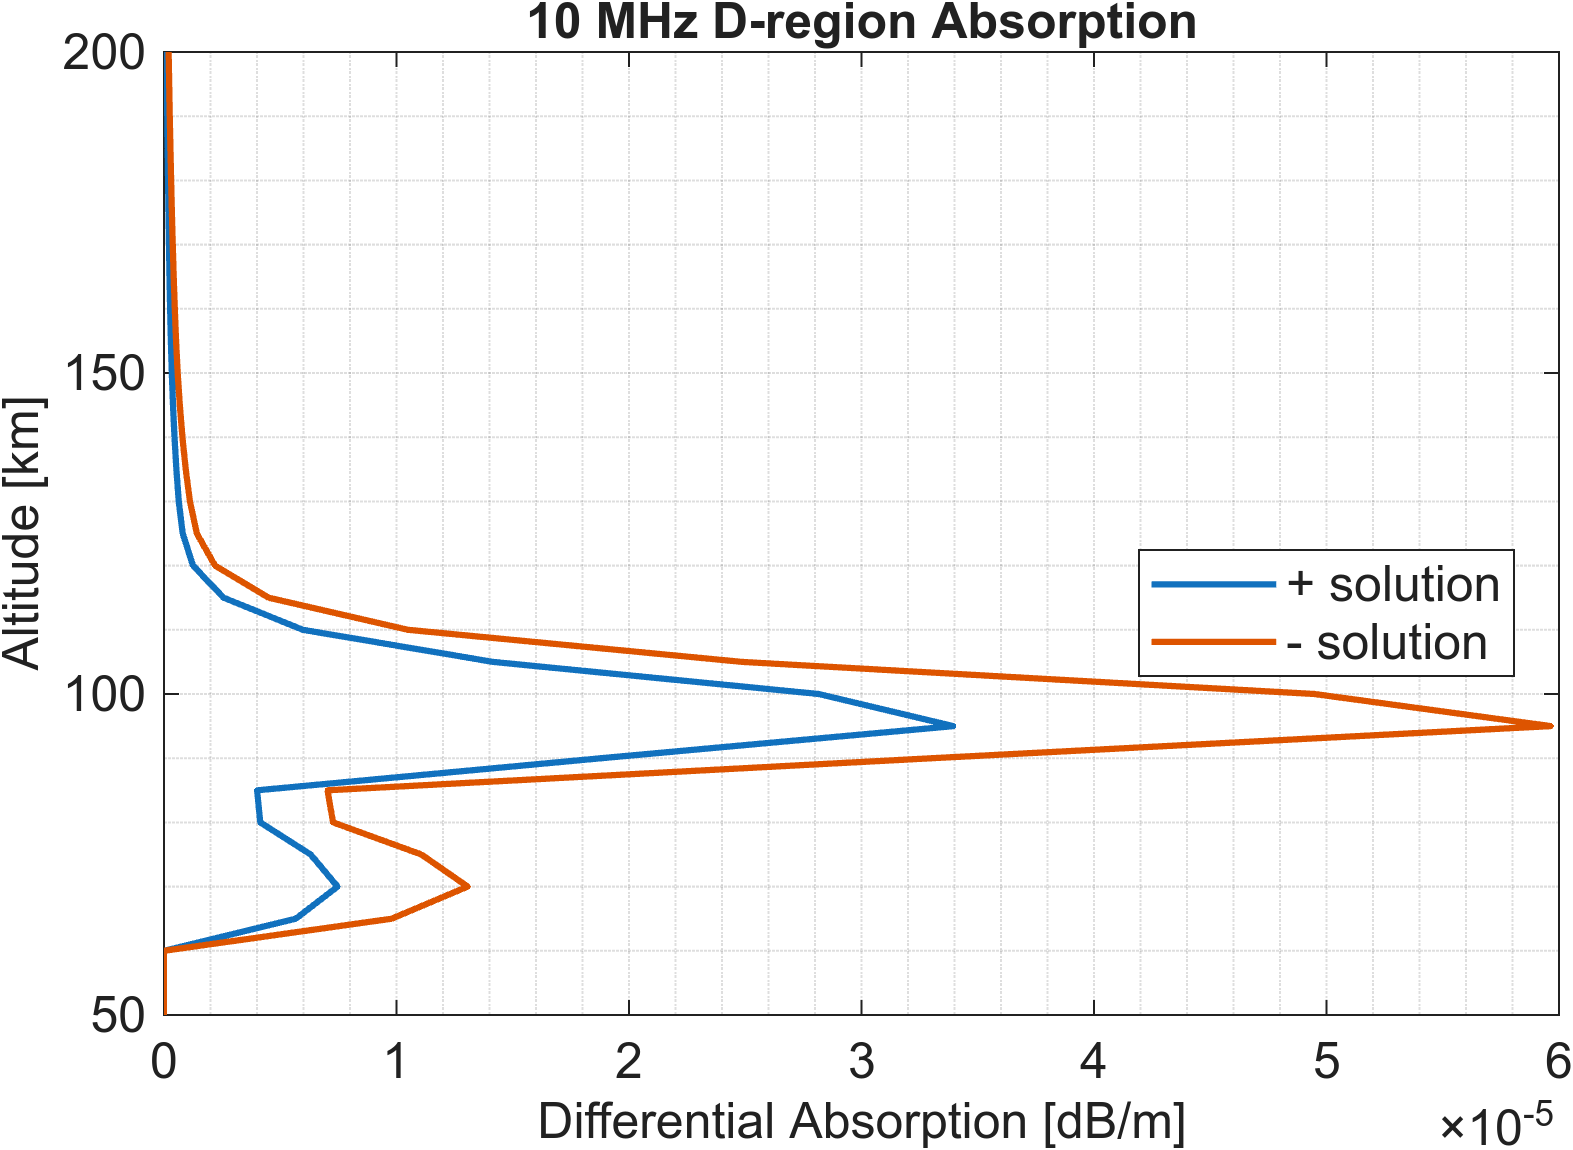
\includegraphics[width=0.6\textwidth]{figures/HW3_P8_absorption_rev.png}
    \caption{10 MHz Differential Absorption}
\end{figure}

\newpage
\section*{Problem 9: ICON Mission}
\hspace*{2em}My favorite instrument aboard ICON would be MIGHTI, built by the Naval Research Laboratory.
Its purpose is to measure the neutral winds and temperatures of the thermosphere between roughly 90 and 300 km.
It's made up of two identical sensors, MIGHTI-A and MIGHTI-B, that look at the Earth with fields of view
perpendicular to each other. Its SWAP is is spread across two sensors, a shared camera
electronics box, and a calibration lamp assembly, but each sensor's baffle is about 62 cm long, the cameras use
roughly 11 to 13 watts, and the calibration lamps weigh about 2.7 kg. It works by observing the red and
green airglow lines of atomic oxygen, which are Doppler shifted when the neutral gas is moving, and
measuring that shift with an interferometer gives the wind along the line of sight. Since MIGHTI-B views the same
patch of atmosphere minutes after MIGHTI-A, the two views are combined into the full horizontal wind vector.
The instrument contributes to ICON's goal of connecting the lower atmosphere to the ionosphere by measuring the neutral winds that
occur, since these winds generate electric fields through the ionosphere and push plasma along the field lines,
which can then be compared with the plasma motion measured by IVM.

\newpage
\section*{MATLAB Code}

\begin{lstlisting}
%% ASEN 5335 Aerospace Environment
%% Justin Le
%% HW3 Problem 1

clc;clear; close all

% Read IRI output
data = readmatrix('iri_output.txt', 'FileType', 'text', 'NumHeaderLines', 30);
data(data == -1) = NaN; % IRI uses -1 for missing values

alt  = data(:,1); % km
Ne   = data(:,2); % cm^-3
pct  = data(:,7:12); % ion percentages of Ne: O+ N+ H+ He+ O2+ NO+

% Set ion number densities [cm^-3]
n_ion = Ne .* pct / 100;
n_Op  = n_ion(:,1);
n_Hp  = n_ion(:,3);
n_Hep = n_ion(:,4);
n_O2p = n_ion(:,5);
n_NOp = n_ion(:,6);

% Consistent ion colors across figures: O+ H+ O2+ NO+ He+
c = lines(5);

% Plotting
figure;
semilogx(Ne,    alt, 'k-',  'LineWidth', 2); hold on
semilogx(n_Op,  alt, 'Color', c(1,:), 'LineWidth', 1.5);
semilogx(n_Hp,  alt, 'Color', c(2,:), 'LineWidth', 1.5);
semilogx(n_O2p, alt, 'Color', c(3,:), 'LineWidth', 1.5);
semilogx(n_NOp, alt, 'Color', c(4,:), 'LineWidth', 1.5);
semilogx(n_Hep, alt, 'Color', c(5,:), 'LineWidth', 1.5);
grid minor
xlabel('Number Density [cm^{-3}]')
ylabel('Altitude [km]')
title('IRI Ion and Electron Densities')
legend('e^-', 'O^+', 'H^+', 'O_2^+', 'NO^+', 'He^+', 'Location', 'best')
set(gcf, 'Units', 'inches', 'Position', [0 0 6 4]);
set(findall(gcf, '-property', 'FontSize'), 'FontSize', 12);
exportgraphics(gcf, fullfile('figures', 'HW3_P1_iri_output.png'), 'Resolution', 900);

% Normalized as percentages
n_plot = [n_Op n_Hp n_O2p n_NOp n_Hep];
pct_norm = 100 * n_plot ./ sum(n_plot, 2, 'omitnan');

figure;
h = plot(pct_norm, alt, 'LineWidth', 1.5);
set(h, {'Color'}, num2cell(c, 2));
grid minor
xlim([0 100])
xlabel('Ion Composition [%]')
ylabel('Altitude [km]')
title('IRI Normalized Ion Composition')
legend('O^+', 'H^+', 'O_2^+', 'NO^+', 'He^+', 'Location', 'best')
set(gcf, 'Units', 'inches', 'Position', [0 0 6 4]);
set(findall(gcf, '-property', 'FontSize'), 'FontSize', 12);
exportgraphics(gcf, fullfile('figures', 'HW3_P1_ion_composition.png'), 'Resolution', 900);

% Total electron content (TEC), 1 TECU = 1e16 el/m^2
TECU = 1e16;
z_m  = alt * 1e3; % m
Ne_m = Ne * 1e6;  % m^-3
Ne_m(isnan(Ne_m)) = 0; % no electrons where IRI has no data

[NmF2, k_pk] = max(Ne); % peak electron density splits topside/bottomside
hmF2 = alt(k_pk);

TEC_total  = trapz(z_m, Ne_m) / TECU
TEC_bottom = trapz(z_m(1:k_pk), Ne_m(1:k_pk)) / TECU
TEC_top    = trapz(z_m(k_pk:end), Ne_m(k_pk:end)) / TECU

100*(TEC_bottom/TEC_total)
100*(TEC_top/TEC_total)
\end{lstlisting}

\newpage
\begin{lstlisting}
%% ASEN 5335 Aerospace Environment
%% Justin Le
%% HW3 Problem 4

clc; clear; close all

% Constants
qe = 1.602176634e-19; % C
kB = 1.380649e-23; % J/K
me = 9.1093837e-31; % kg
mi = 1.67262192e-27; % kg, H+ at GEO

% GEO plasma
n = 0.5e6; % cm^-3 -> m^-3
T = 5e6; % K, Te = Ti
kT = kB * T / qe; % thermal voltage [V]
fprintf('kT/q = %.1f V\n', kT);

% Thermal velocities [m/s]
ve = sqrt(3 * kB * T / me);
vi = sqrt(3 * kB * T / mi);

% Photocurrent (Eq. 28), surface normal to sun
Jph0 = 40e-6; % A/m^2
kTph = 2; % eV

% Random current densities at V = 0 if areas cancel out
Je0 = 0.25*qe*n*ve;
Ji0 = 0.25*qe*n*vi;

% Shadow surface: dQ/dt = Ie + Ii = 0, V < 0
V_neg = linspace(-10*kT, 0, 1e5); % V
dQ_shadow = -Je0*exp(V_neg/kT) + Ji0*(1 - V_neg/kT);
k = find(dQ_shadow < 0, 1, 'first'); % first sign change in net current
V_shadow = interp1(dQ_shadow(k-1:k), V_neg(k-1:k), 0);
fprintf('Shadow potential = %.1f V (%.2f kTe)\n', V_shadow, V_shadow/kT);

% Sunlit surface: dQ/dt = Ie + Ii + Iph = 0, V > 0
V_pos = linspace(0, 100, 1e5); % V
dQ_sun = -Je0*(1 + V_pos/kT) + Ji0*exp(-V_pos/kT) + Jph0*exp(-V_pos/kTph);
k = find(dQ_sun < 0, 1, 'first'); % first sign change in net current
V_sun = interp1(dQ_sun(k-1:k), V_pos(k-1:k), 0);
fprintf('Sunlit potential = %.2f V\n', V_sun);

% Differential charging
dV = V_sun - V_shadow;
fprintf('Potential difference = %.1f V\n', dV);
\end{lstlisting}

\newpage
\begin{lstlisting}
%% ASEN 5335 Aerospace Environment
%% Justin Le
%% HW3 Problem 5

clc; clear; close all

% Read IRI output
data = readmatrix('iri_output.txt', 'FileType', 'text', 'NumHeaderLines', 30);
data(data == -1) = NaN; % IRI uses -1 for missing values

alt = data(:,1); % km
Ne  = data(:,2); % cm^-3
Ne(isnan(Ne)) = 0;

% Critical frequency profile [MHz], Module 3 Eq. 31 (n_e in cm^-3)
fc = 9e-3 * sqrt(Ne);

% (i) Critical frequency foF2 = minimum frequency to reach space
[foF2, k_pk] = max(fc);
hmF2 = alt(k_pk);
fprintf('foF2 = %.2f MHz at %.0f km\n', foF2, hmF2);

% (iii) Reflection altitude of a 2 MHz wave: first altitude where fc = f
f = 2; % MHz
k = find(fc >= f, 1, 'first');
z_reflect = interp1(fc(k-1:k), alt(k-1:k), f);
fprintf('2 MHz reflects at %.1f km\n', z_reflect);

% Topside reflection altitude: last altitude where fc = f (space-to-ground)
k2 = find(fc >= f, 1, 'last');
z_reflect_top = interp1(fc(k2:k2+1), alt(k2:k2+1), f);
fprintf('2 MHz reflects on the topside at %.1f km\n', z_reflect_top);

% Plot critical frequency profile
figure;
plot(fc, alt, 'k-', 'LineWidth', 2); hold on
xline(f, 'r--', '2 MHz', 'LineWidth', 1.5);
yline(z_reflect, 'b--', sprintf('%.0f km', z_reflect), 'LineWidth', 1.5);
yline(z_reflect_top, 'b--', sprintf('%.0f km', z_reflect_top), 'LineWidth', 1.5);
grid minor
xlabel('Critical Frequency [MHz]')
ylabel('Altitude [km]')
title('IRI Critical Frequency Profile')
set(gcf, 'Units', 'inches', 'Position', [0 0 6 4]);
set(findall(gcf, '-property', 'FontSize'), 'FontSize', 12);
exportgraphics(gcf, fullfile('figures', 'HW3_P5_plasma_freq_rev.png'), 'Resolution', 300)
\end{lstlisting}

\newpage
\begin{lstlisting}
%% ASEN 5335 Aerospace Environment
%% Justin Le
%% HW3 Problem 8

clc; clear; close all
addpath(fullfile('..', 'HW2')) % MSISatmosphere1000.m

% Read IRI output
data = readmatrix('iri_output.txt', 'FileType', 'text', 'NumHeaderLines', 30);
data(data == -1) = NaN; % IRI uses -1 for missing values

alt = data(:,1); % km
Ne  = data(:,2) * 1e6; % Convert cm^-3 to m^-3
Ne(isnan(Ne)) = 0; % no electrons where IRI has no data

% Neutral densities from MSIS [cm^-3]
msis = MSISatmosphere1000(alt);
n_n  = msis.n2 + msis.o2 + msis.o;

% Neutral density at the surface [cm^-3]
msis0 = MSISatmosphere1000(0);
n_n0  = msis0.n2 + msis0.o2 + msis0.o;

% Electron-neutral collision frequency [s^-1], nu_en = 1.2e11 N/N0
nu = 1.2e11 * n_n ./ n_n0;

% Constants
qe = 1.602176634e-19; % C
me = 9.1093837e-31; % kg
B0 = 50000e-9; % T

% Wave and gyro frequencies [rad/s]
f   = 10e6; % Hz
w   = 2*pi*f;
w_c = qe * B0 / me;
fprintf('f_H = %.2f MHz\n', w_c/(2*pi*1e6));

% Differential absorption [dB/m] for + (w + w_c) and - (w - w_c) solutions
dAdl_plus = 4.6e-5 * Ne .* nu ./ (nu.^2 + (w + w_c)^2);
dAdl_minus = 4.6e-5 * Ne .* nu ./ (nu.^2 + (w - w_c)^2);

% Total attenuation along vertical path [dB]
z_m = alt * 1e3; % m
A_plus = trapz(z_m, dAdl_plus);
A_minus = trapz(z_m, dAdl_minus);
fprintf('A+ attenuation = %.2f dB\n', A_plus);
fprintf('A- attenuation = %.2f dB\n', A_minus);

% Plot differential absorption profile
figure;
plot(dAdl_plus, alt, 'LineWidth', 1.5); hold on
plot(dAdl_minus, alt, 'LineWidth', 1.5);
grid minor
ylim([50 200])
xlabel('Differential Absorption [dB/m]')
ylabel('Altitude [km]')
title('10 MHz D-region Absorption')
legend('+ solution', '- solution', 'Location', 'best')
set(gcf, 'Units', 'inches', 'Position', [0 0 6 4]);
set(findall(gcf, '-property', 'FontSize'), 'FontSize', 12);
exportgraphics(gcf, fullfile('figures', 'HW3_P8_absorption_rev.png'), 'Resolution', 300)
\end{lstlisting}


\end{document}
